\chapter{Introduction}

\section{Dataset Shift}


In the field of machine learning and predictive modeling, it is often assumed that data distributions remain static, meaning they do not change between the training and deployment phases of the model. However, in practice, this assumption is rarely satisfied: data distributions can undergo significant changes between the training and testing scenarios.

This phenomenon is known as \curlyquotes{\textbf{dataset shift}}\cite{shiftbook} and is closely related to another field of study, referred to by various terms such as \curlyquotes{\textbf{transfer learning}} or \curlyquotes{\textbf{inductive transfer}}. Transfer learning addresses the problem of how information can be drawn from a number of only partially related training scenarios and used to provide better predictions in one of those scenarios compared to using only that specific scenario. Therefore, dataset shift represents a more specific case: it deals with relating information in, typically, two closely related environments to improve prediction in one given the dataset in the other. Given this issue, it is crucial to develop an understanding of the suitability of particular models under such changing conditions, and it is necessary to consider whether a different predictive model should be employed.

Among the various forms of dataset shift, covariate shift, studied and described by Shimodaira\cite{SHIMODAIRA2000227}, is one of the most extensively researched. It encompasses situations where the distribution of the covariates, $P(X)$ changes, while the conditional relationship $P(Y \mid X)$, representing the relationship between the covariates $X$ and the target $Y$, remains unchanged. In this case, the typical values of the covariates observed during testing differ from those observed during training.

	
\subsection{Most common causes of dataset shift}
	
The two most common and well-studied causes of dataset shift are:

\begin{enumerate}
	\item Sample selection bias
	\item Non-stationary environments
\end{enumerate}

\textbf{Sample selection bias} occurs when there is a discrepancy in the data distribution due to the training data being obtained through a biased method, and therefore not reliably representing the real environment in which the classifier will be used (the test set). This bias is not necessarily a flaw of the algorithm or data management process but a systematic defect in the way the data is collected or labeled, causing a non-uniform selection of training examples from the population. This often leads to bias being introduced during training. Dataset shift resulting from sample selection bias is particularly relevant when dealing with imbalanced classification problems, as, in highly imbalanced domains, the minority class is especially sensitive to misclassification errors due to its typically low number of samples.

In real-world applications, data often is not stationary (in time or space). One of the most relevant \textbf{non-stationary} scenarios involves adversarial classification problems, such as spam filtering and network intrusion detection.
	

\section{Simple Covariate Shift}

The most fundamental form of dataset shift, known as \textit{covariate shift}, can be formally defined as follows. Consider an input variable \( X \) and a response variable \( Y \), where \( X \to Y \) represents the relationship between the two. Let \( P_{\text{tra}} \) denote the probability distribution of the training data and \( P_{\text{tst}} \) denote the probability distribution of the test data. A covariate shift occurs when:  
\[
P_{\text{tra}}(Y \mid X) = P_{\text{tst}}(Y \mid X) \quad \text{but} \quad P_{\text{tra}}(X) \neq P_{\text{tst}}(X)\,.
\]

In other words, the conditional distribution of \( Y \) given \( X \) remains unchanged across training and test datasets, while the marginal distribution of \( X \) differs. \cref{fig:covariate-shift} shows an example of different distribution between training data and test data, creating a division between the two datasets.  
	
\begin{figure}[H]
	\centering
	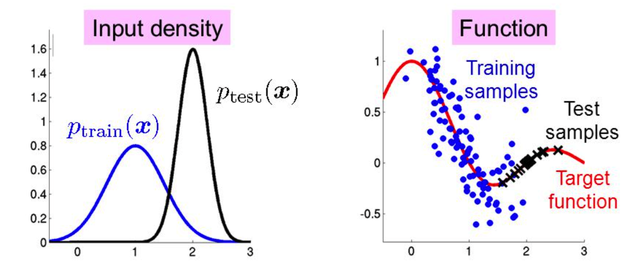
\includegraphics[width=0.8\textwidth]{assets/immagine.png} 
	\caption{Example of covariate shift.}
	\label{fig:covariate-shift}
\end{figure}

This phenomenon can affect a wide range of machine learning models, regardless of the task they are designed to perform. It is commonly encountered in scenarios where models classify data or predict trends based on input features. This issue is particularly relevant in diverse machine learning applications, including but not limited to:
	
	\begin{enumerate}
		\item Image categorization and facial recognition systems
		\item Speech recognition and translation software
		\item Diagnostic and screening tools in healthcare
	\end{enumerate}
	
For example, consider a model designed to distinguish between cats and dogs. Our training data might consist of images like those shown in \cref{fig:cani-gatti} (top). At test time, we are asked to classify the images from the test set as the one in the bottom of the same figure. Once deployed, the model will not accurately distinguish between cats and dogs because the feature distribution will differ. Model may achieve a high degree of accuracy on a labeled training dataset, identifying and classifying the object in an image. However, when deployed with real-time data, changes in the input distribution can significantly impact the model's accuracy.

\begin{figure}[H]
	\centering
	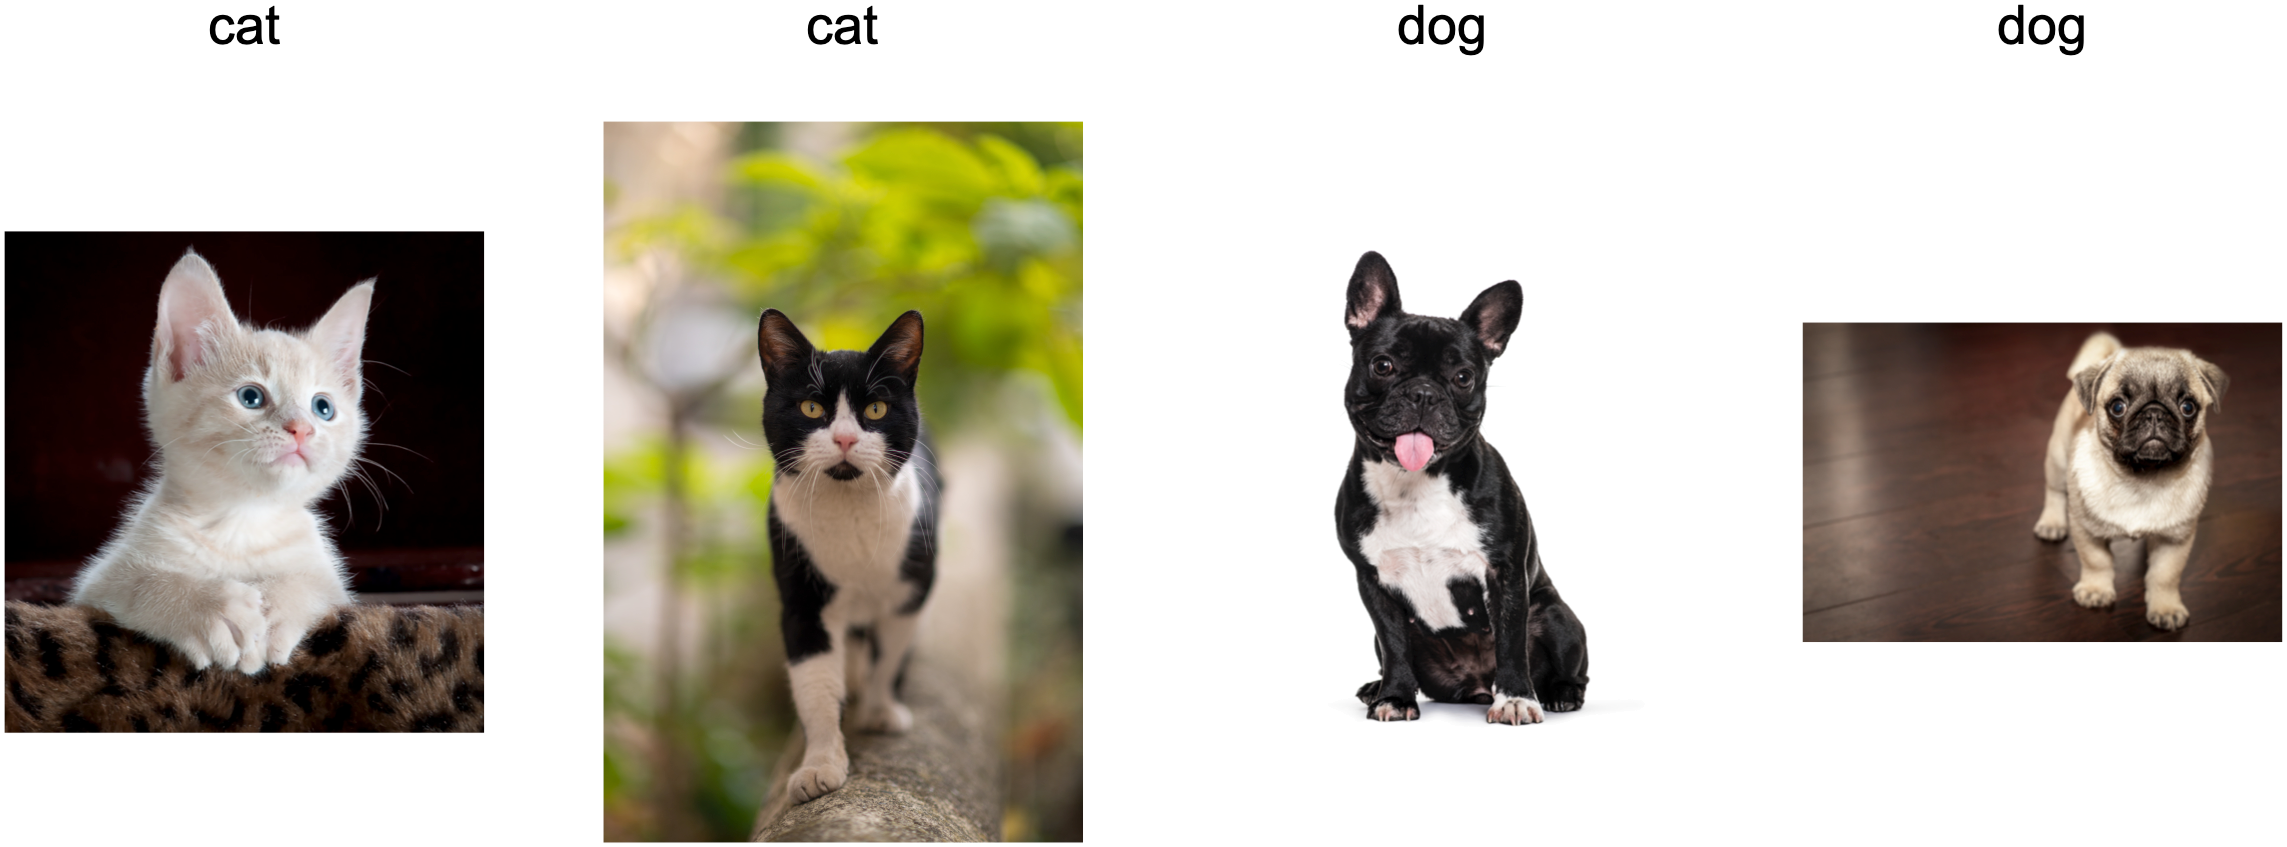
\includegraphics[width=0.65\textwidth]{assets/cat-dog-train.png}
	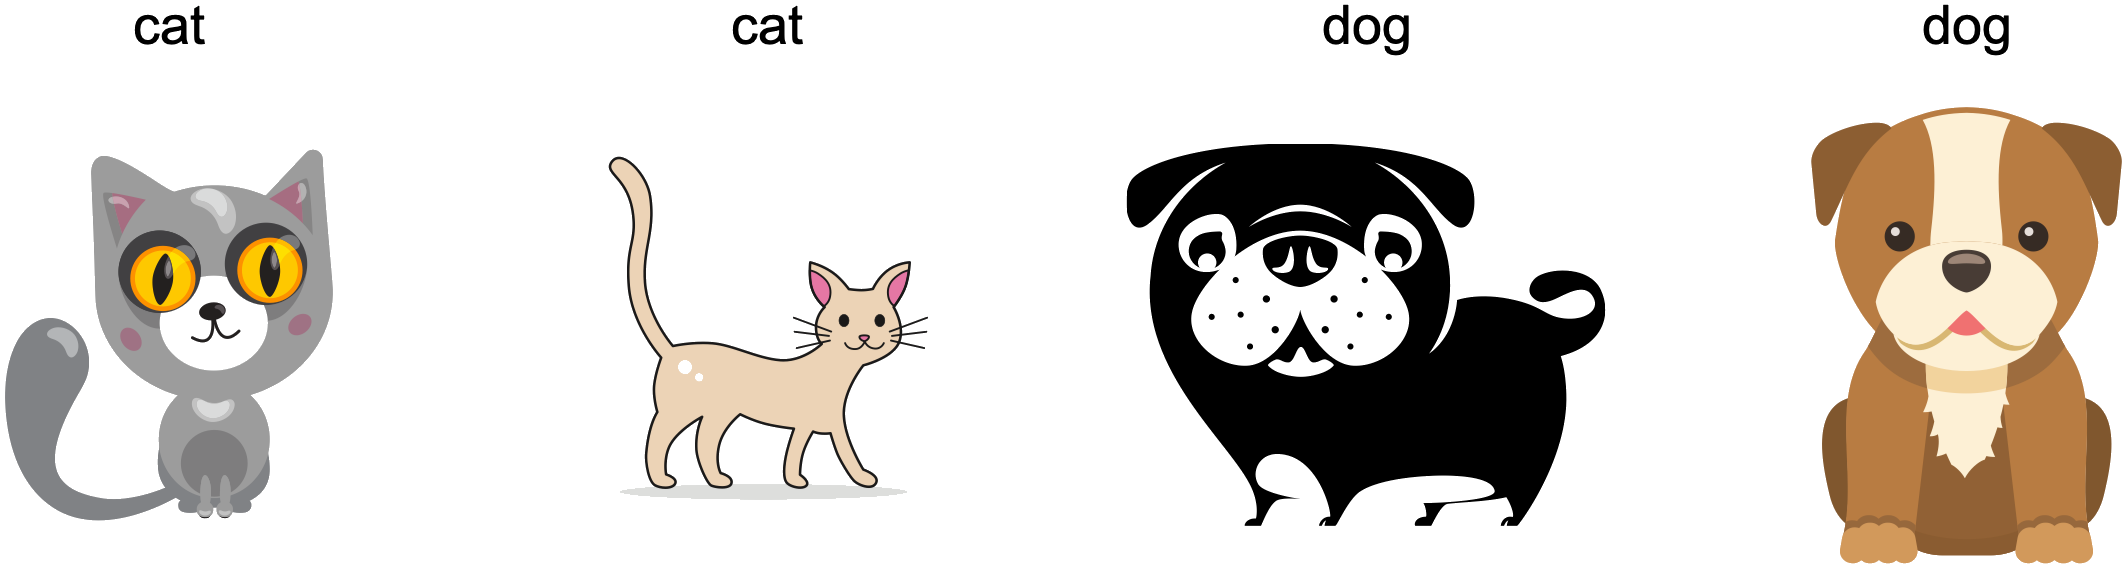
\includegraphics[width=0.65\textwidth]{assets/cat-dog-test.png} 
	\caption{Training (top) and testing (bottom) data for distinguishing cats and dogs.}
	\label{fig:cani-gatti}
\end{figure}

The same can accure in facial recognition: the training data might not include subjects from specific ethnicities or age groups. When the model is deployed in a real-world environment, subjects that do not align with the training data may exhibit an unrecognizable feature distribution. Another cause of covariate shift could be variations in environmental conditions, such as lighting. For instance, an image categorization model trained under specific lighting conditions may perform poorly when deployed in an operational setting with different lighting.
	
Supervised learning models are typically trained on labeled data, which is prepared and curated by data scientists to ensure high quality through outlier detection and analysis. However, this level of control is not feasible in operational environments, as input data becomes unpredictable once the model is deployed. Consequently, the training data often differs in distribution from real-world input data, both in availability and characteristics. This mismatch can negatively impact the model's accuracy. Trained algorithms may fail to recognize features from a different data distribution, leading to reduced performance or even complete ineffectiveness, as illustrated in \cref{fig:inaccurate-model}. This highlights a critical issue in machine learning: a model that performs well on training data may not retain its accuracy post-deployment.

The primary objective is to assess the extent of the covariate shift, implement mitigation strategies, and enhance the model's accuracy. Addressing covariate shift also reveals the model's generalization ability: its capacity to apply learned features from training data to unseen data. Poor generalization often stems from overfitting, where the model becomes overly tailored to the training data, making it ineffective for inputs with differing distributions.

\begin{figure}[H]
	\centering
	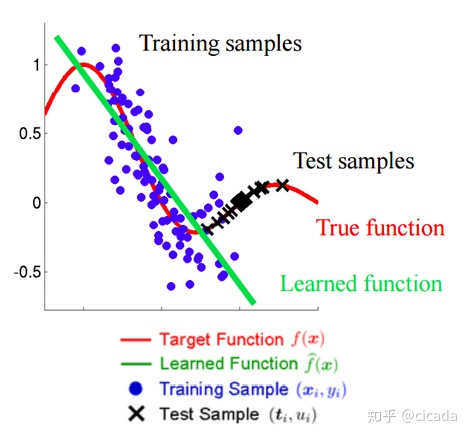
\includegraphics[width=0.55\textwidth]{assets/covariate_shift.png} 
	\caption{Example of inaccurate model.}
	\label{fig:inaccurate-model}
\end{figure}
